% !TeX program = xelatex
\documentclass[a4paper,10pt]{article}

% ============================================================================
% កញ្ចប់បណ្ណាល័យ (Packages) – តាមលំនាំស្តង់ដារ អនុវិទ្យាល័យព្រះក្រសាំង (ls_plan.tex)
% បរិបទ៖ ថ្នាក់រៀនគ្មានស្លាយ LCD – បង្រៀនដោយប្រើក្ដារខៀន បន្ទាត់ក្រិត ដែកឈាន អេគែរ និងសន្លឹកកិច្ចការស-ខ្មៅ
% ============================================================================
\usepackage[a4paper, left=0.95cm, right=0.95cm, top=0.85cm, bottom=0.92cm, footskip=0.52cm]{geometry}
\usepackage{amsmath}
\usepackage{unicode-math}
\usepackage{fontspec}
\usepackage{array, longtable, multirow, colortbl}
\usepackage[table]{xcolor}
\usepackage{enumitem}
\usepackage{pifont}
\usepackage{fancyhdr}
\usepackage{tikz}
\usetikzlibrary{calc, arrows.meta, angles, quotes, decorations.markings, positioning, babel}

\makeatletter
\let\@expl@@@mark@update@singlecol@structures@@\relax
\makeatother

% ============================================================================
% ការកំណត់ពុម្ពអក្សរផ្លូវការ (Cross-Platform Fonts Configuration)
% ============================================================================
\providecommand{\NGSFindFonts}{%
  \IfFileExists{C:/Windows/Fonts/cambria.ttc}{%
    \def\NGSSysPath{C:/Windows/Fonts/}%
    \def\NGSUserPath{C:/Users/KIT/AppData/Local/Microsoft/Windows/Fonts/}%
  }{%
    \IfFileExists{./fonts/KhmerOSsiemreap.ttf}{\def\NGSSysPath{./fonts/}\def\NGSUserPath{./fonts/}}{%
    \IfFileExists{../fonts/KhmerOSsiemreap.ttf}{\def\NGSSysPath{../fonts/}\def\NGSUserPath{../fonts/}}{%
    \IfFileExists{../../fonts/KhmerOSsiemreap.ttf}{\def\NGSSysPath{../../fonts/}\def\NGSUserPath{../../fonts/}}{%
    \IfFileExists{../../../fonts/KhmerOSsiemreap.ttf}{\def\NGSSysPath{../../../fonts/}\def\NGSUserPath{../../../fonts/}}{%
    \IfFileExists{../../../../fonts/KhmerOSsiemreap.ttf}{\def\NGSSysPath{../../../../fonts/}\def\NGSUserPath{../../../../fonts/}}{%
    \IfFileExists{../../../../../fonts/KhmerOSsiemreap.ttf}{\def\NGSSysPath{../../../../../fonts/}\def\NGSUserPath{../../../../../fonts/}}{%
    \IfFileExists{../../../../../../fonts/KhmerOSsiemreap.ttf}{\def\NGSSysPath{../../../../../../fonts/}\def\NGSUserPath{../../../../../../fonts/}}{%
      \def\NGSSysPath{../../../../../../../fonts/}\def\NGSUserPath{../../../../../../../fonts/}%
    }}}}}}}%
  }%
}
\NGSFindFonts

\setmathfont[Path={\NGSSysPath}, FontIndex=1, Scale=1.02]{cambria.ttc}
\defaultfontfeatures{Ligatures=TeX}

\setmainfont[
  Path={\NGSUserPath},
  Extension=.ttf,
  Script=Khmer,
  BoldFont={KhmerOSsiemreap},
  BoldFeatures={FakeBold=1.8},
  ItalicFont={KhmerOSsiemreap},
  ItalicFeatures={FakeSlant=0.25},
  BoldItalicFont={KhmerOSsiemreap},
  BoldItalicFeatures={FakeBold=1.8, FakeSlant=0.25}
]{KhmerOSsiemreap}

\newfontfamily\muol[Path={\NGSUserPath}, Extension=.ttf, Script=Khmer]{KhmerOSmuollight}
\newfontfamily\TimesEn[Path={\NGSSysPath}, Extension=.ttf, BoldFont={timesbd}, ItalicFont={timesi}, BoldItalicFont={timesbi}]{times}
\newfontfamily\NagaBold[Path={\NGSUserPath}, Extension=.ttf]{AKbalthom Naga Bold}
\newfontfamily\CalibriFont[Path={\NGSSysPath}, Extension=.ttf]{calibri}
\newfontfamily\Tacteing[Path={\NGSUserPath}]{TACTENG.TTF}
\newfontfamily\CourierBullet[Path={\NGSSysPath}, Extension=.ttf]{cour}
\newcommand{\wcirc}{{\CourierBullet\fontsize{9.5pt}{11pt}\selectfont o}}

\XeTeXlinebreaklocale "km"
\XeTeXlinebreakskip = 0pt plus 1pt minus 0.1pt

\definecolor{stepgray}{HTML}{D9D9D9}
\definecolor{headgray}{HTML}{F2F2F2}
\definecolor{boxgray}{HTML}{D9D9D9}
\definecolor{darkred}{HTML}{C00000}
\definecolor{red5e}{HTML}{FF0000}

\pagestyle{fancy}
\fancyhf{}
\renewcommand{\headrulewidth}{0pt}
\fancyfoot[R]{\CalibriFont\fontsize{11pt}{13pt}\selectfont\thepage}

\setlength{\parindent}{0pt}
\setlength{\parskip}{0pt}
\setlength{\tabcolsep}{3.8pt}

\newcolumntype{L}[1]{>{\raggedright\arraybackslash}p{#1}}

\newcommand{\en}[1]{{\TimesEn #1}}
\newcommand{\enbf}[1]{{\TimesEn\textbf{#1}}}
\newcommand{\unit}[1]{\,\text{\en{#1}}}
\newcommand{\fiveE}[1]{{\NagaBold\fontsize{9.5pt}{13pt}\selectfont\textcolor{red5e}{#1}}}
\newcommand{\timenote}[1]{\textcolor{darkred}{\textit{#1}}}
\newcommand{\graybox}[1]{\colorbox{boxgray}{\strut\hspace{2pt}#1\hspace{2pt}}}
\newcommand{\ditem}{\tikz[baseline=-0.5ex]\fill (0,0.42ex) -- (0.42ex,0) -- (0,-0.42ex) -- (-0.42ex,0) -- cycle;\hspace{0.3em}}
\newcommand{\cnum}[1]{{\fontsize{10.5pt}{12pt}\selectfont\ding{\numexpr171+#1\relax}}\hspace{0.2em}}
\newcommand{\cfig}[1]{\par\vspace{4pt}{\centering #1\par}\vspace{4pt}}
\newcommand{\stepheader}[1]{\multicolumn{3}{|c|}{\cellcolor{stepgray}\muol #1} \\* \noalign{\hrule height 0.4pt}}
\newcommand{\tri}[1]{\ensuremath{\triangle #1}}
\newcommand{\ang}[1]{\ensuremath{\angle #1}}
\newcommand{\arc}[1]{\ensuremath{\widehat{#1}}}
\newcommand{\cg}{\ensuremath{\cong}}
\newcommand{\khmflourish}{{\Tacteing\fontsize{36pt}{14pt}\selectfont\raisebox{-5pt}{3}}}

\tikzset{
  tk1/.style={postaction={decorate},decoration={markings,mark=at position 0.50 with {\draw[black, line width=0.85pt](0,-0.095)--(0,0.095);}}},
  tk2/.style={postaction={decorate},decoration={markings,
    mark=at position 0.45 with {\draw[black, line width=0.85pt](0,-0.095)--(0,0.095);},
    mark=at position 0.55 with {\draw[black, line width=0.85pt](0,-0.095)--(0,0.095);}}}
}

% ============================================================================
% ម៉ាក្រូរូបភាពធរណីមាត្រស-ខ្មៅ (Proportional 4.2–7.2 cm B&W TikZ Diagrams)
% ============================================================================

% ១. កំណែលំហាត់ទី៥ (ទំ.២០៤) + E1 Engage ទទឹងផ្ទៃទឹកក្នុងលូបេតុងរាងរង្វង់
\newcommand{\figEngageCIRCFour}{%
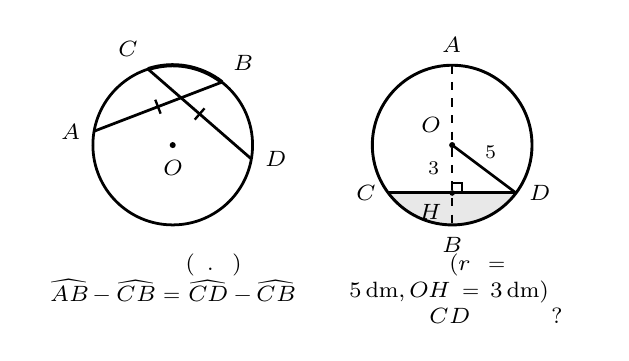
\begin{tikzpicture}[scale=0.78, every node/.style={font=\footnotesize, text=black}]
  % ឆ្វេង៖ កំណែលំហាត់ទី៥ ទំ.២០៤ (AB = CD => ដកធ្នូរួម CB បាន ធ្នូ AC = ធ្នូ BD)
  \begin{scope}[shift={(0,0)}]
    \coordinate (O) at (1.55,1.40);
    \draw[black, line width=1.0pt] (O) circle (1.30);
    \coordinate (A) at ($(O)+(170:1.30)$);
    \coordinate (C) at ($(O)+(108:1.30)$);
    \coordinate (B) at ($(O)+(52:1.30)$);
    \coordinate (D) at ($(O)+(-10:1.30)$);
    \draw[black, line width=1.0pt, tk1] (A)--(B);
    \draw[black, line width=1.0pt, tk1] (C)--(D);
    \draw[black, line width=1.45pt] (B) arc (52:108:1.30);
    \fill[black] (O) circle (1.4pt) node[below=2pt] {$O$};
    \node[left=1.5pt] at (A) {$A$};
    \node[above left=1pt] at (C) {$C$};
    \node[above right=1pt] at (B) {$B$};
    \node[right=1.5pt] at (D) {$D$};
    \node[anchor=north, text width=3.45cm, align=center] at (1.55,-0.22) {កំណែលំហាត់ទី៥ (ទំ.២០៤)៖\\$\arc{AB}-\arc{CB}=\arc{CD}-\arc{CB}$};
  \end{scope}
  % ស្ដាំ៖ បេសកកម្ម E1 ទទឹងផ្ទៃទឹកក្នុងលូបេតុងរាងរង្វង់ (r=5 dm, OH=3 dm => CD=?)
  \begin{scope}[shift={(4.50,0)}]
    \coordinate (O) at (1.60,1.40);
    % ផ្ទៃទឹកខាងក្រោមអង្កត់ធ្នូ CD (y = 1.40 - 0.78 = 0.62)
    \begin{scope}
      \clip (O) circle (1.30);
      \fill[gray!18] (0.20,0.05) rectangle (3.00,0.62);
    \end{scope}
    \draw[black, line width=1.05pt] (O) circle (1.30);
    \coordinate (A) at ($(O)+(90:1.30)$);
    \coordinate (B) at ($(O)+(-90:1.30)$);
    \coordinate (C) at (0.56,0.62);
    \coordinate (D) at (2.64,0.62);
    \coordinate (H) at (1.60,0.62);
    \draw[black, line width=1.10pt] (C)--(D);
    \draw[black, line width=0.85pt, dashed] (A)--(B);
    \draw[black, line width=0.95pt] (O)--(D);
    \draw[black, line width=0.75pt] ($(H)+(0,0.16)$) -- ($(H)+(0.16,0.16)$) -- ($(H)+(0.16,0)$);
    \fill[black] (O) circle (1.4pt) node[above left=1pt] {$O$};
    \fill[black] (H) circle (1.3pt) node[below left=1pt] {$H$};
    \node[above=1pt] at (A) {$A$};
    \node[below=1pt] at (B) {$B$};
    \node[left=1.5pt] at (C) {$C$};
    \node[right=1.5pt] at (D) {$D$};
    \node[above right=0pt] at (1.98,1.02) {\scriptsize $5$};
    \node[left=1pt] at (1.60,1.02) {\scriptsize $3$};
    \node[anchor=north, text width=3.55cm, align=center] at (1.60,-0.22) {លូបេតុង ($r=5\unit{dm}, OH=3\unit{dm}$)៖\\តើទទឹងផ្ទៃទឹក $CD$ ស្មើប៉ុន្មាន?};
  \end{scope}
\end{tikzpicture}}

% ២. E3 Explain: លំហាត់គំរូទី១ (AB កែង CD => HC = HD, ទំ.២០៣) និងលំហាត់គំរូទី២ (AB // CD => ធ្នូ AC = ធ្នូ BD, ទំ.២០៣)
\newcommand{\figSymmetryCIRCFour}{%
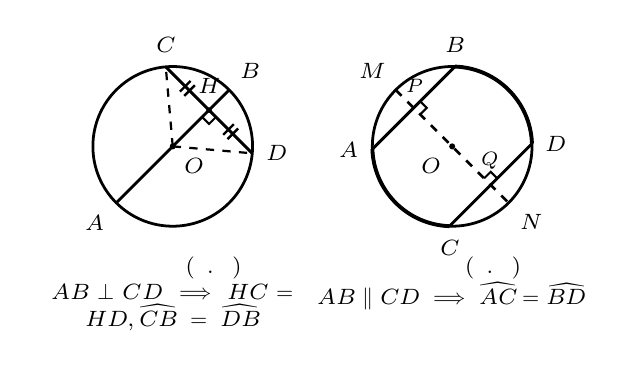
\begin{tikzpicture}[scale=0.78, every node/.style={font=\footnotesize, text=black}]
  % ឆ្វេង៖ លំហាត់គំរូទី១ ទំ.២០៣ (អង្កត់ផ្ចិត AB កែងអង្កត់ធ្នូ CD ត្រង់ H)
  \begin{scope}[shift={(0,0)}]
    \coordinate (O) at (1.55,1.40);
    \draw[black, line width=1.0pt] (O) circle (1.30);
    \coordinate (A) at ($(O)+(225:1.30)$);
    \coordinate (B) at ($(O)+(45:1.30)$);
    \coordinate (C) at ($(O)+(95:1.30)$);
    \coordinate (D) at ($(O)+(-5:1.30)$);
    \coordinate (H) at ($(A)!(C)!(B)$);
    \draw[black, line width=1.05pt] (A)--(B);
    \draw[black, line width=1.05pt] (C)--(D);
    \draw[black, line width=0.85pt, tk2] (C)--(H);
    \draw[black, line width=0.85pt, tk2] (H)--(D);
    \draw[black, line width=0.80pt, dashed] (O)--(C) (O)--(D);
    % សញ្ញាមុំកែងត្រង់ H (បង្វិល 45°)
    \draw[black, line width=0.75pt] ($(H)+(225:0.16)$) -- ($(H)+(225:0.16)+(-45:0.16)$) -- ($(H)+(-45:0.16)$);
    \fill[black] (O) circle (1.4pt) node[below right=1pt] {$O$};
    \fill[black] (H) circle (1.3pt) node[above=2.5pt] {$H$};
    \node[below left=1pt] at (A) {$A$};
    \node[above right=1pt] at (B) {$B$};
    \node[above=1.5pt] at (C) {$C$};
    \node[right=1.5pt] at (D) {$D$};
    \node[anchor=north, text width=3.45cm, align=center] at (1.55,-0.24) {លំហាត់គំរូទី១ (ទំ.២០៣)៖\\$AB\perp CD \implies HC=HD, \arc{CB}=\arc{DB}$};
  \end{scope}
  % ស្ដាំ៖ លំហាត់គំរូទី២ ទំ.២០៣ (អង្កត់ធ្នូស្រប AB // CD កាត់ដោយអង្កត់ផ្ចិតកែង MN)
  \begin{scope}[shift={(4.50,0)}]
    \coordinate (O) at (1.60,1.40);
    \draw[black, line width=1.0pt] (O) circle (1.30);
    \coordinate (M) at ($(O)+(135:1.30)$);
    \coordinate (N) at ($(O)+(-45:1.30)$);
    \coordinate (A) at ($(O)+(182:1.30)$);
    \coordinate (B) at ($(O)+(88:1.30)$);
    \coordinate (C) at ($(O)+(-92:1.30)$);
    \coordinate (D) at ($(O)+(2:1.30)$);
    \coordinate (P) at ($(M)!(A)!(N)$);
    \coordinate (Q) at ($(M)!(C)!(N)$);
    \draw[black, line width=0.95pt, dashed] (M)--(N);
    \draw[black, line width=1.05pt] (A)--(B) (C)--(D);
    \draw[black, line width=1.40pt] (A) arc (182:268:1.30);
    \draw[black, line width=1.40pt] (D) arc (2:88:1.30);
    \draw[black, line width=0.75pt] ($(P)+(-45:0.15)$) -- ($(P)+(-45:0.15)+(45:0.15)$) -- ($(P)+(45:0.15)$);
    \draw[black, line width=0.75pt] ($(Q)+(135:0.15)$) -- ($(Q)+(135:0.15)+(45:0.15)$) -- ($(Q)+(45:0.15)$);
    \fill[black] (O) circle (1.4pt) node[below left=1pt] {$O$};
    \node[above left=1pt] at (M) {$M$};
    \node[below right=1pt] at (N) {$N$};
    \node[left=1.5pt] at (A) {$A$};
    \node[above=1.5pt] at (B) {$B$};
    \node[below=1.5pt] at (C) {$C$};
    \node[right=1.5pt] at (D) {$D$};
    \node[above=2pt] at (P) {\scriptsize $P$};
    \node[above=2pt] at (Q) {\scriptsize $Q$};
    \node[anchor=north, text width=3.50cm, align=center] at (1.60,-0.24) {លំហាត់គំរូទី២ (ទំ.២០៣)៖\\$AB \parallel CD \implies \arc{AC} = \arc{BD}$};
  \end{scope}
\end{tikzpicture}}

% ៣. E4 & E5: លំហាត់ទី៤ (ទំ.២០៤ អង្កត់ធ្នូស្មើចម្ងាយ OQ = OR) + ប្រតិបត្តិ (ទំ.២០៣ អង្កត់ផ្ចិត AD និង AB // CD)
\newcommand{\figPracticeCIRCFour}{%
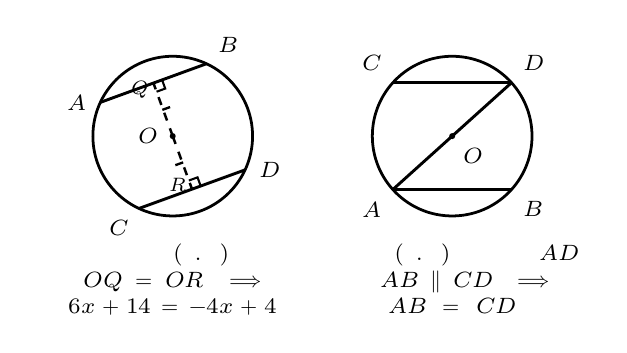
\begin{tikzpicture}[scale=0.78, every node/.style={font=\footnotesize, text=black}]
  % ឆ្វេង៖ លំហាត់ទី៤ ទំ.២០៤ (OQ = OR => AB = CD, 6x+14 = -4x+4)
  \begin{scope}[shift={(0,0)}]
    \coordinate (O) at (1.55,1.40);
    \draw[black, line width=1.0pt] (O) circle (1.30);
    \coordinate (A) at ($(O)+(155:1.30)$);
    \coordinate (B) at ($(O)+(65:1.30)$);
    \coordinate (C) at ($(O)+(-115:1.30)$);
    \coordinate (D) at ($(O)+(-25:1.30)$);
    \coordinate (Q) at ($(A)!0.5!(B)$);
    \coordinate (R) at ($(C)!0.5!(D)$);
    \draw[black, line width=1.05pt] (A)--(B) (C)--(D);
    \draw[black, line width=0.90pt, dashed, tk1] (O)--(Q);
    \draw[black, line width=0.90pt, dashed, tk1] (O)--(R);
    \draw[black, line width=0.75pt] ($(Q)+(-70:0.15)$) -- ($(Q)+(-70:0.15)+(20:0.15)$) -- ($(Q)+(20:0.15)$);
    \draw[black, line width=0.75pt] ($(R)+(110:0.15)$) -- ($(R)+(110:0.15)+(20:0.15)$) -- ($(R)+(20:0.15)$);
    \fill[black] (O) circle (1.4pt) node[left=2pt] {$O$};
    \node[left=1.5pt] at (A) {$A$};
    \node[above right=1pt] at (B) {$B$};
    \node[below left=1pt] at (C) {$C$};
    \node[right=1.5pt] at (D) {$D$};
    \node at ($(Q)+(205:0.24)$) {\scriptsize $Q$};
    \node at ($(R)+(165:0.24)$) {\scriptsize $R$};
    \node[anchor=north, text width=3.45cm, align=center] at (1.55,-0.20) {លំហាត់ទី៤ (ទំ.២០៤)៖\\$OQ=OR \implies 6x+14=-4x+4$};
  \end{scope}
  % ស្ដាំ៖ ប្រតិបត្តិ ទំ.២០៣ (អង្កត់ផ្ចិត AD និង AB // CD => AB = CD)
  \begin{scope}[shift={(4.50,0)}]
    \coordinate (O) at (1.60,1.40);
    \draw[black, line width=1.0pt] (O) circle (1.30);
    \coordinate (A) at ($(O)+(222:1.30)$);
    \coordinate (B) at ($(O)+(-42:1.30)$);
    \coordinate (C) at ($(O)+(138:1.30)$);
    \coordinate (D) at ($(O)+(42:1.30)$);
    \draw[black, line width=1.05pt] (A)--(D);
    \draw[black, line width=1.05pt] (A)--(B) (C)--(D);
    \fill[black] (O) circle (1.4pt) node[below right=1pt] {$O$};
    \node[below left=1pt] at (A) {$A$};
    \node[below right=1pt] at (B) {$B$};
    \node[above left=1pt] at (C) {$C$};
    \node[above right=1pt] at (D) {$D$};
    \node[anchor=north, text width=3.50cm, align=center] at (1.60,-0.20) {ប្រតិបត្តិ (ទំ.២០៣)៖ អង្កត់ផ្ចិត $AD$\\និង $AB\parallel CD \implies AB = CD$};
  \end{scope}
\end{tikzpicture}}

\begin{document}
\fontsize{10pt}{15.2pt}\selectfont

% -------------------- ក្បាលកិច្ចតែងការ (Header) --------------------
\begin{center}
  {\muol\fontsize{11pt}{16pt}\selectfont ព្រះរាជាណាចក្រកម្ពុជា}\\[2pt]
  {\muol\fontsize{10pt}{15pt}\selectfont ជាតិ សាសនា ព្រះមហាក្សត្រ}\\[1pt]
  \khmflourish
\end{center}

\vspace{-28pt}
{\muol\fontsize{9.5pt}{12.5pt}\selectfont
មន្ទីរអប់រំ យុវជន និងកីឡា ខេត្តកំពង់ធំ\\
ការិយាល័យអប់រំ យុវជន និងកីឡា ស្រុកកំពង់ស្វាយ\\
អនុវិទ្យាល័យព្រះក្រសាំង}

\vspace{1pt}
\begin{center}
  {\muol\fontsize{10pt}{14pt}\selectfont កិច្ចតែងការបង្រៀន}
\end{center}
\vspace{0pt}

% -------------------- ព័ត៌មានទូទៅ (Metadata) --------------------
{\renewcommand{\arraystretch}{0.95}
\hspace*{4.05cm}%
\begin{tabular}{@{}l l l@{}}
  - \hspace{0.35cm} មុខវិជ្ជា & : & គណិតវិទ្យា ថ្នាក់ទី៨ \\
  - \hspace{0.35cm} ចំណងជើងមេរៀន & : & មេរៀនទី១៥ រង្វង់ \\
  - \hspace{0.35cm} ចំណងជើងរង & : & ២.២ លក្ខណៈឆ្លុះនៃរង្វង់ (សៀវភៅសិក្សាគោល ទំ.២០២--២០៤) \\
  - \hspace{0.35cm} រយៈពេល & : & ១ ម៉ោងសិក្សា (៥០ នាទី) \\
  - \hspace{0.35cm} បង្រៀនដោយ & : & ហុក ប៊ុនថែន \\
  - \hspace{0.35cm} កាលបរិច្ឆេទ & : & ថ្ងៃចន្ទ ៤រោច ខែមិគសិរ ព.ស.២៥៧០ (២៨ ធ្នូ ២០២៦) \\
\end{tabular}
}

\vspace{1pt}

% -------------------- I. វត្ថុបំណង --------------------
\textbf{I.} {\muol វត្ថុបំណង}\\[1pt]
\hspace*{0.55cm}%
\begin{tabular}{@{}l l L{14.2cm}@{}}
  \wcirc \hspace{0.25cm} វិជ្ជាសម្បទា & : & សិស្សពោលបានត្រឹមត្រូវនូវលក្ខណៈឆ្លុះទាំងបួននៃរង្វង់៖ ផ្ចិតឆ្លុះ $O$ អ័ក្សឆ្លុះជាអង្កត់ផ្ចិត ទ្រឹស្ដីបទអង្កត់ផ្ចិតកែងនឹងអង្កត់ធ្នូ ($AB\perp CD \implies HC=HD$ និង $\arc{CB}=\arc{DB}$) ធ្នូចន្លោះអង្កត់ធ្នូស្របគ្នា ($AB\parallel CD \implies \arc{AC}=\arc{BD}$) និងលក្ខណៈអង្កត់ធ្នូស្មើចម្ងាយពីផ្ចិត ($OQ=OR \iff AB=CD$) តាមសៀវភៅគោល ទំ.២០២--២០៤ ។ \\
  \wcirc \hspace{0.25cm} បំណិនសម្បទា & : & សិស្សគូស \textbf{អង្កត់ផ្ចិតជំនួយកែងនឹងអង្កត់ធ្នូ} ដើម្បីស្រាយបញ្ជាក់ធ្នូស្មើគ្នា អនុវត្តទ្រឹស្ដីបទពីតាករក្នុងត្រីកោណកែងកាំ-ចម្ងាយផ្ចិត ($r^2 = OH^2 + HD^2$) និងដោះស្រាយសមីការប្រវែងអង្កត់ធ្នូលើសន្លឹកកិច្ចការស-ខ្មៅបានត្រឹមត្រូវ ។ \\
  \wcirc \hspace{0.25cm} ចរិយាសម្បទា & : & សិស្សមានទម្លាប់ផ្ទៀងផ្ទាត់លក្ខខណ្ឌប្រវែងវិជ្ជមានក្រោយដោះស្រាយសមីការពិជគណិតក្នុងធរណីមាត្រ និងឃើញតម្លៃអនុវត្តនៃអង្កត់ផ្ចិតកែងអង្កត់ធ្នូក្នុងការវាស់ទទឹងផ្ទៃទឹកក្នុងលូ និងសំណង់បំពង់មូល ។ \\
\end{tabular}

\vspace{1pt}

% -------------------- II. សម្ភារៈឧបទេស --------------------
\textbf{II.} {\muol សម្ភារៈឧបទេស}\\[1pt]
\hspace*{0.55cm}$\bullet$ \hspace{0.35cm} សៀវភៅសិក្សាគោលគណិតវិទ្យាថ្នាក់ទី៨ (ទំ.២០២--២០៤) ក្ដារខៀន ដីស បន្ទាត់ក្រិត ដែកឈាន អេគែរ (បន្ទាត់កែង) និងសន្លឹកកិច្ចការសិស្សស-ខ្មៅ (\en{Worksheet\_CIRC4} ចំនួន ២ ទំព័រ \en{A4} ដោយគ្មានស្លាយ \en{LCD}) ។

\vspace{1pt}

% -------------------- III. វិធីសាស្រ្តបង្រៀន --------------------
\textbf{III.} {\muol វិធីសាស្រ្តបង្រៀន}\\[1pt]
\hspace*{0.55cm}$\bullet$ \hspace{0.35cm} គោលវិធីសិស្សមជ្ឈមណ្ឌលតាមគំរូ \en{5Es} រួមបញ្ចូល \textbf{វិធីឆ្លុះអ័ក្សតាមអង្កត់ផ្ចិតកែង} (\en{Diameter Axial-Symmetry Reasoning}, \en{Guti\'errez et al., 2021}) និង \textbf{ការភ្ជាប់រូបភាព-ពិជគណិតលើអង្កត់ធ្នូស្មើចម្ងាយ} (\en{Zazkis et al., 1996}) ។

\vspace{2pt}

% -------------------- IV. ដំណើរការបង្រៀន --------------------
\textbf{IV.} {\muol ដំណើរការបង្រៀន}\\[-6pt]

{\renewcommand{\arraystretch}{1.15}
\begin{longtable}{|L{5.50cm}|L{7.90cm}|L{4.80cm}|}
\hline
\multicolumn{1}{|c|}{\cellcolor{headgray}\muol សកម្មភាពគ្រូ} &
\multicolumn{1}{c|}{\cellcolor{headgray}\muol ខ្លឹមសារមេរៀន} &
\multicolumn{1}{c|}{\cellcolor{headgray}\muol សកម្មភាពសិស្ស} \\[2pt]
\hline
\endfirsthead

\hline
\multicolumn{1}{|c|}{\cellcolor{headgray}\muol សកម្មភាពគ្រូ} &
\multicolumn{1}{c|}{\cellcolor{headgray}\muol ខ្លឹមសារមេរៀន} &
\multicolumn{1}{c|}{\cellcolor{headgray}\muol សកម្មភាពសិស្ស} \\[2pt]
\hline
\endhead

\hline
\endfoot

% ==================== ជំហានទី១ (2min) ====================
\stepheader{ជំហានទី១ ៖ រដ្ឋបាលថ្នាក់ (២ នាទី)}
$\bullet$ ពិនិត្យអវត្តមាន សណ្ដាប់ធ្នាប់ អនាម័យ និងការត្រៀមបន្ទាត់ក្រិត-អេគែរ \par\vspace{1pt}
$\bullet$ ចែកសន្លឹកកិច្ចការស-ខ្មៅ \en{Worksheet\_CIRC4} (១ សន្លឹកសងខាងក្នុងម្នាក់)
&
$\bullet$ វត្តមានសិស្ស វិន័យ និងការត្រៀមបន្ទាត់ក្រិត ដែកឈាន និងអេគែរ \par\vspace{1pt}
$\bullet$ សន្លឹកកិច្ចការសិស្ស \en{Worksheet\_CIRC4} (មេរៀនទី១៥ ៖ ២.២ លក្ខណៈឆ្លុះនៃរង្វង់)
&
$\circ$ ប្រធានថ្នាក់រាយការណ៍អវត្តមាន \par\vspace{1pt}
$\circ$ ទទួលសន្លឹកកិច្ចការ សរសេរឈ្មោះ និងដាក់បន្ទាត់-អេគែរលើតុ \\
\hline

% ==================== ជំហានទី២ (9min) ====================
\stepheader{ជំហានទី២ ៖ កែកិច្ចការផ្ទះ រំលឹកមេរៀនចាស់ និងភ្ជាប់បញ្ហាថ្មី (៩ នាទី)}
\timenote{(កែកិច្ចការផ្ទះ $\le 3\unit{min}$)} \par
$\bullet$ ហៅសិស្ស ១ នាក់ឡើងបង្ហាញសម្រាយបញ្ជាក់លំហាត់ទី៥ (ទំ.២០៤) លើក្ដារខៀន
&
\textbf{កំណែកិច្ចការផ្ទះ (លំហាត់ទី៥ ទំ.២០៤)៖} \par
$\bullet$ ដោយអង្កត់ធ្នូ $AB = CD \implies$ ធ្នូ $\arc{AB} = \arc{CD}$ (ទ្រឹស្ដីបទច្រាសអង្កត់ធ្នូស្មើគ្នា) ។ \par
$\bullet$ ដកធ្នូរួម $\arc{CB}$ ពីអង្គទាំងពីរ៖ $\arc{AB} - \arc{CB} = \arc{CD} - \arc{CB} \implies \boxed{\arc{AC} = \arc{BD}}$ ។
&
$\circ$ ផ្ទៀងផ្ទាត់សម្រាយបញ្ជាក់ដកធ្នូរួម $\arc{CB}$ ក្នុងសៀវភៅលំហាត់ \\[3pt]

\timenote{(រំលឹកមេរៀនទាក់ទង $3\unit{min}$)} \par
$\bullet$ សួររំលឹកនិយមន័យ \textbf{មេដ្យាទ័រ (អ័ក្សឆ្លុះនៃអង្កត់)} និង \textbf{ទ្រឹស្ដីបទពីតាករ} ក្នុងត្រីកោណកែង
&
\textbf{រំលឹកចំណេះដឹងមូលដ្ឋានភ្ជាប់មេរៀនថ្មី៖} \par
១. \textbf{បម្លែងឆ្លុះធៀបនឹងបន្ទាត់ $d$៖} $P'$ ឆ្លុះនឹង $P$ ធៀបនឹង $d \iff d$ ជាមេដ្យាទ័រនៃអង្កត់ $PP'$ ($d\perp PP'$ ត្រង់ចំណុចកណ្ដាល) ។ \par
២. \textbf{ទ្រឹស្ដីបទពីតាករ៖} ក្នុង $\tri{OHD}$ កែងត្រង់ $H$ មាន $OD^2 = OH^2 + HD^2$ ។
&
$\circ$ ឆ្លើយរំលឹកលក្ខណៈមេដ្យាទ័រ និងរូបមន្តពីតាករ $OD^2 = OH^2 + HD^2$ \\[3pt]

\fiveE{E1 - Engage} \timenote{(3 min)} \par
$\bullet$ លើកបញ្ហា \textbf{«ទទឹងផ្ទៃទឹកក្នុងលូបេតុងរាងរង្វង់»} លើក្ដារខៀន និងផ្នែកទី១ នៃសន្លឹកកិច្ចការ \par
\hspace*{0.3em}– សំណួរ៖ «បើលូមូលមានកាំ $r = 5\unit{dm}$ ហើយផ្ទៃទឹកស្ថិតនៅចម្ងាយកែង $OH = 3\unit{dm}$ ក្រោមផ្ចិត $O$ តើទទឹងផ្ទៃទឹក $CD$ ស្មើនឹង $4\unit{dm}$ ឬ $8\unit{dm}$?»
&
\textbf{បេសកកម្ម E1 ៖ វាស់ទទឹងផ្ទៃទឹកក្នុងលូបេតុងមូល ($r = 5\unit{dm}$)} \par
ជាងសំណង់ពិនិត្យលូបេតុងរាងរង្វង់កាំ $OD = 5\unit{dm}$ ។ ផ្ទៃទឹកផ្ដេកបង្កើតបានអង្កត់ធ្នូ $CD$ ដែលស្ថិតនៅចម្ងាយកែង $OH = 3\unit{dm}$ ពីផ្ចិត $O$ ។ \par
$\bullet$ \textbf{មតិទី១៖} តាមពីតាករឃើញ $4\unit{dm}$ ដូច្នេះទទឹងផ្ទៃទឹក $CD = 4\unit{dm}$ ។ \par
$\bullet$ \textbf{មតិទី២៖} $HD = 4\unit{dm}$ គ្រាន់តែជាពាក់កណ្ដាលអង្កត់ធ្នូប៉ុណ្ណោះ ឯទទឹងផ្ទៃទឹកពេញគឺ $CD = 2\times 4 = \mathbf{8\unit{dm}}$ ។
&
$\circ$ អានបេសកកម្មលើសន្លឹកកិច្ចការ និងគូសធីកទស្សន៍ទាយមតិទី១ ឬមតិទី២ \\[3pt]

&
\cfig{\figEngageCIRCFour}
& \\[3pt]
\hline

% ==================== ជំហានទី៣ (17min) ====================
\stepheader{ជំហានទី៣ ៖ មេរៀនថ្មី — លក្ខណៈឆ្លុះនៃរង្វង់ (១៧ នាទី)}
\fiveE{E2 - Explore} \timenote{(11 min)} \par
\ditem \textbf{សកម្មភាពទី១៖ អ័ក្សឆ្លុះ និងអង្កត់ផ្ចិតកែងអង្កត់ធ្នូលើរូបខ្នាតពិត $1:1$ ($5.5\unit{min}$)} \par
$\bullet$ ឱ្យដៃគូសិស្សពិនិត្យផ្ចិតឆ្លុះ $O$ និងអ័ក្សឆ្លុះអង្កត់ផ្ចិត (ឧទាហរណ៍ទី១--៣ ទំ.២០២)
&
\textbf{១. រុករកផ្ចិតឆ្លុះ អ័ក្សឆ្លុះ និងអង្កត់ផ្ចិតកែងអង្កត់ធ្នូ (ទំ.២០២--២០៣)៖} \par
$\bullet$ \textbf{ឧទាហរណ៍ទី១--៣ (ទំ.២០២)៖} គ្រប់ចំណុច $B$ លើរង្វង់មានចំណុចឆ្លុះ $B'$ ធៀបនឹង $O$ លើរង្វង់ ($OB=OB'=r$) ហើយរាល់ចំណុចឆ្លុះ $P'$ ធៀបនឹងអង្កត់ផ្ចិត $AB$ ក៏ស្ថិតលើរង្វង់ដែរ ($OP'=OP=r$) $\implies O$ ជា \textbf{ផ្ចិតឆ្លុះ} ឯគ្រប់អង្កត់ផ្ចិតជា \textbf{អ័ក្សឆ្លុះ} ។
&
$\circ$ សង្កេតឃើញការបត់រង្វង់តាមអង្កត់ផ្ចិតណាមួយធ្វើឱ្យកន្លះរង្វង់ទាំងពីរត្រួតស៊ីគ្នា \\[3pt]

$\bullet$ ឱ្យសិស្សប្រើបន្ទាត់ក្រិតវាស់លើរូប ក ខ្នាតពិត $1:1$ ($r = 1.5\unit{cm}, OH = 0.9\unit{cm}$ ក្នុងផ្នែកទី២ នៃសន្លឹកកិច្ចការ) រួចប្រៀបធៀប $HC$ និង $HD$
&
$\bullet$ \textbf{វាស់លើរូប ក ខ្នាតពិត $1:1$ ($r=1.5\unit{cm}, OH=0.9\unit{cm}$)៖} \par
\hspace*{0.3em}– វាស់ឃើញ $HC = \mathbf{1.2\unit{cm}}$ និង $HD = \mathbf{1.2\unit{cm}} \implies HC = HD$ ($CD = 2.4\unit{cm}$) ។ \par
\hspace*{0.3em}– \textbf{សម្រាយតាមត្រីកោណកែង៖} ក្នុង $\tri{OHC}$ និង $\tri{OHD}$ កែងត្រង់ $H$ មានអ៊ីប៉ូតេនុស $OC=OD=r$ និងជ្រុងរួម $OH \implies \tri{OHC}\cg\tri{OHD}$ $\implies \mathbf{HC = HD}$ និង $\ang{COH}=\ang{DOH} \implies \arc{CB}=\arc{DB}$ ។
&
$\circ$ ប្រើបន្ទាត់ក្រិតវាស់ឃើញ $HC = HD = 1.2\unit{cm}$ និងផ្ទៀង $0.9^2 + 1.2^2 = 1.5^2$ \\[3pt]

\ditem \textbf{សកម្មភាពទី២៖ អង្កត់ធ្នូស្របគ្នា និងអង្កត់ធ្នូស្មើចម្ងាយពីផ្ចិត ($5.5\unit{min}$)} \par
$\bullet$ ឱ្យសិស្សពិនិត្យរូប ខ ($AB \parallel CD$)៖ បើគូសអង្កត់ផ្ចិតជំនួយ $MN \perp AB$ តើ $MN$ កែងនឹង $CD$ ដែរឬទេ?
&
\textbf{២. រុករកធ្នូចន្លោះអង្កត់ធ្នូស្រប និងអង្កត់ធ្នូស្មើចម្ងាយពីផ្ចិត៖} \par
$\bullet$ \textbf{ករណី $AB \parallel CD$ (លំហាត់គំរូទី២ ទំ.២០៣)៖} គូសអង្កត់ផ្ចិតជំនួយ $MN \perp AB$ ត្រង់ $P \implies MN \perp CD$ ត្រង់ $Q$ ដែរ ។ ធៀបនឹងអ័ក្សឆ្លុះ $MN$ ចំណុច $A$ ឆ្លុះនឹង $B$ ហើយ $C$ ឆ្លុះនឹង $D \implies \boxed{\arc{AC} = \arc{BD}}$ ។
&
$\circ$ គូសអង្កត់ផ្ចិតជំនួយ $MN\perp AB$ និងបំពេញជំហានឆ្លុះអ័ក្សលើសន្លឹកកិច្ចការ \\[3pt]

$\bullet$ សួរបន្ត៖ «ចុះបើចម្ងាយកែងពីផ្ចិត $OQ = OR$ តើប្រវែងអង្កត់ធ្នូ $AB$ និង $CD$ យ៉ាងដូចម្ដេច?»
&
$\bullet$ \textbf{ករណីចម្ងាយកែងស្មើគ្នា ($OQ = OR$)៖} តាមពីតាករ $QB = \sqrt{r^2 - OQ^2}$ និង $RD = \sqrt{r^2 - OR^2}$ ។ ដូចនេះ $OQ = OR \iff QB = RD \iff \mathbf{AB = CD}$ ។
&
$\circ$ ទាញបានសមមូល $OQ=OR \iff AB=CD$ តាមទ្រឹស្ដីបទពីតាករ \\[3pt]

\fiveE{E3 - Explain} \timenote{(6 min)} \par
$\bullet$ សំយោគប្រអប់ \textbf{ជាទូទៅ} ទាំង ៤ ចំណុច (ទំ.២០២) និងទ្រឹស្ដីបទពាក់ព័ន្ធ (ទំ.២០៣--២០៤) លើក្ដារខៀន
&
{\muol ២.២ លក្ខណៈឆ្លុះនៃរង្វង់ — ជាទូទៅ (សៀវភៅគោល ទំ.២០២--២០៣)} \par
$\bullet$ រង្វង់មាន \textbf{ផ្ចិតឆ្លុះ} មួយគឺ ចំណុចផ្ចិត $O$ របស់វា ហើយ \textbf{គ្រប់អង្កត់ផ្ចិតទាំងអស់} ជា \textbf{អ័ក្សឆ្លុះ} នៃរង្វង់ ។ \par
$\bullet$ \textbf{អង្កត់ផ្ចិតកែងនឹងអង្កត់ធ្នូ (លំហាត់គំរូទី១ ទំ.២០៣)៖} បើអង្កត់ផ្ចិត $AB \perp CD$ ត្រង់ $H$ នោះវាចែកអង្កត់ធ្នូ និងធ្នូស្កាត់ជាពីរផ្នែកប៉ុនគ្នា ($HC = HD$, $\arc{CB}=\arc{DB}$, $\arc{CA}=\arc{DA}$) ។
&
$\circ$ បំពេញប្រអប់ជាទូទៅផ្នែកខាងលើក្នុងផ្នែកទី៣ នៃសន្លឹកកិច្ចការ \\[3pt]

$\bullet$ សង្កត់ធ្ងន់លក្ខខណ្ឌច្រាស \textit{(អង្កត់ធ្នូមិនមែនអង្កត់ផ្ចិត)} និងធ្នូចន្លោះអង្កត់ធ្នូស្របគ្នា
&
$\bullet$ \textbf{ច្រាសមកវិញ (ទំ.២០២)៖} អង្កត់ផ្ចិតដែលកាត់តាមចំណុចកណ្ដាលនៃអង្កត់ធ្នូ \textit{(មិនមែនអង្កត់ផ្ចិត)} កែងនឹងអង្កត់ធ្នូនោះ ហើយចែកធ្នូសន្ធឹងជាពីរផ្នែកប៉ុនគ្នា ។ \par
$\bullet$ \textbf{ធ្នូចន្លោះអង្កត់ធ្នូស្រប (លំហាត់គំរូទី២ ទំ.២០៣)៖} បើអង្កត់ធ្នូ $AB \parallel CD$ នោះ $\arc{AC} = \arc{BD}$ ។
&
$\circ$ កត់សម្គាល់ការប្រុងប្រយ័ត្ន៖ អង្កត់ផ្ចិតពីរកាត់ចែកគ្នាត្រង់ $O$ មិនចាំបាច់កែងគ្នាទេ \\[3pt]

&
\cfig{\figSymmetryCIRCFour}
& \\[3pt]

$\bullet$ សង្ខេបធនាគារហេតុផល \cnum{1}--\cnum{5} សម្រាប់លក្ខណៈឆ្លុះ និងចម្ងាយអង្កត់ធ្នូពីផ្ចិត
&
{\fontsize{9.2pt}{13pt}\selectfont
\begin{tabular}[t]{|L{7.55cm}|}
\hline
\cellcolor{headgray}\textbf{ធនាគារហេតុផល (\en{Warrant Bank}) សម្រាប់លក្ខណៈឆ្លុះនៃរង្វង់} \\[2pt]
\hline
\cnum{1} អ័ក្សឆ្លុះនៃរង្វង់៖ គ្រប់អង្កត់ផ្ចិតជាអ័ក្សឆ្លុះនៃរង្វង់ ឯផ្ចិត $O$ ជាផ្ចិតឆ្លុះ \par
\cnum{2} អង្កត់ផ្ចិតកែងអង្កត់ធ្នូ៖ $AB\perp CD \implies HC=HD = \tfrac{1}{2}CD$ និង $\arc{CB}=\arc{DB}$ \par
\cnum{3} អង្កត់ផ្ចិតកាត់ចំណុចកណ្ដាលអង្កត់ធ្នូ ($CD$ មិនមែនអង្កត់ផ្ចិត)៖ $HC=HD \implies AB\perp CD$ \par
\cnum{4} អង្កត់ធ្នូស្របគ្នា៖ $AB \parallel CD \implies$ ធ្នូចន្លោះ $\arc{AC} = \arc{BD}$ (ឆ្លុះតាមអង្កត់ផ្ចិតកែង $MN$) \par
\cnum{5} ចម្ងាយពីផ្ចិតទៅអង្កត់ធ្នូ៖ $OQ = OR \iff AB = CD$ និង $r^2 = OH^2 + \left(\tfrac{CD}{2}\right)^2$ \\[2pt]
\hline
\end{tabular}}\par\vspace{2pt}
&
$\circ$ ផ្ទៀងផ្ទាត់លេខកូដហេតុផល \cnum{1}--\cnum{5} លើសន្លឹកកិច្ចការ \\
\hline

% ==================== ជំហានទី៤ (20min) ====================
\stepheader{ជំហានទី៤ ៖ ពង្រឹងចំណេះដឹង និងវាយតម្លៃ (២០ នាទី)}
\fiveE{E4 - Elaborate} \timenote{(10 min)} \par
\ditem \textbf{គំរូទី១៖ លំហាត់គំរូទី២ សៀវភៅគោល ទំ.២០៣ ($4.5\unit{min}$)} \par
$\bullet$ ណែនាំឱ្យសិស្សគូសអង្កត់ផ្ចិតជំនួយ $MN \perp AB$ សម្រាប់បង្ហាញថា $\arc{AC}=\arc{BD}$
&
\textbf{គំរូទី១ (លំហាត់គំរូទី២ ទំ.២០៣ — ធ្នូចន្លោះអង្កត់ធ្នូស្របគ្នា)៖} \par
ក្នុងរង្វង់ផ្ចិត $O$ គេមានអង្កត់ធ្នូ $AB \parallel CD$ ។ ស្រាយបញ្ជាក់ថាធ្នូ $\arc{AC} = \arc{BD}$ ។ \par
$\bullet$ គូសអង្កត់ផ្ចិតជំនួយ $MN \perp AB$ ត្រង់ $P$ ។ ដោយ $AB \parallel CD \implies MN \perp CD$ ត្រង់ $Q$ ដែរ ។
&
$\circ$ គូសអង្កត់ផ្ចិតជំនួយកែង $MN$ កាត់ $AB$ និង $CD$ ត្រង់ $P$ និង $Q$ \\[3pt]

$\bullet$ ឱ្យសិស្សទាញផលវិបាកនៃការឆ្លុះអ័ក្សតាមអង្កត់ផ្ចិត $MN$ ក្នុងផ្នែកទី៤ នៃសន្លឹកកិច្ចការ
&
$\bullet$ តាម \cnum{1} និង \cnum{2} អង្កត់ផ្ចិត $MN$ ជាអ័ក្សឆ្លុះនៃរង្វង់ និងជាមេដ្យាទ័រនៃ $AB$ និង $CD$ ($AP=BP, CQ=DQ$) នាំឱ្យ $A$ ឆ្លុះនឹង $B$ ហើយ $C$ ឆ្លុះនឹង $D$ ធៀបនឹង $MN$ ។ \par
$\bullet$ ដូចនេះ ធ្នូ $\arc{AC}$ និងធ្នូ $\arc{BD}$ ឆ្លុះគ្នាធៀបនឹងអង្កត់ផ្ចិត $MN \implies \boxed{\arc{AC} = \arc{BD}}$ ។
&
$\circ$ បំពេញជំហានឆ្លុះអ័ក្សទាញបាន $\arc{AC}=\arc{BD}$ លើសន្លឹកកិច្ចការ \\[3pt]

\ditem \textbf{គំរូទី២៖ លំហាត់ទី៤ សៀវភៅគោល ទំ.២០៤ — អង្កត់ធ្នូស្មើចម្ងាយពីផ្ចិត ($5.5\unit{min}$)} \par
$\bullet$ ដឹកនាំសិស្សបង្កើតសមីការពី $OQ = OR$ រកតម្លៃ $x$ រួចផ្ទៀងផ្ទាត់ប្រវែងអង្កត់ធ្នូ $AB$ និង $CD$
&
\textbf{គំរូទី២ (លំហាត់ទី៤ ទំ.២០៤ — គណនាប្រវែង $AB$ និង $CD$)៖} \par
ក្នុងរង្វង់ផ្ចិត $O$ គេមានចម្ងាយកែង $OQ = OR$ ហើយ $AB = 6x + 14$ និង $CD = -4x + 4$ ។ \par
$\bullet$ ដោយ $OQ = OR$ ($OQ\perp AB, OR\perp CD$) តាម \cnum{5} គេបានអង្កត់ធ្នូ $AB = CD$៖ \par
\hspace*{0.3em}$6x + 14 = -4x + 4 \implies 6x + 4x = 4 - 14 \implies 10x = -10 \implies \mathbf{x = -1}$ ។ \par
$\bullet$ ជំនួស $x = -1$ រកប្រវែង៖ $AB = 6(-1) + 14 = \mathbf{8}$ និង $CD = -4(-1) + 4 = \mathbf{8}$ ($> 0$ ផ្ទៀងផ្ទាត់!) ។
&
$\circ$ ដោះស្រាយសមីការរកឃើញ $x = -1$ និងជំនួសផ្ទៀងផ្ទាត់បាន $AB = CD = 8$ \\[3pt]

&
\cfig{\figPracticeCIRCFour}
& \\[3pt]

$\bullet$ \textbf{សំណួរឆ្លុះបញ្ចាំង (\en{EIA Looking-Back})៖} \par
\hspace*{0.3em}– សួរ៖ «ហេតុអ្វីបានជាតម្លៃ $x = -1$ (អវិជ្ជមាន) នៅតែជាចម្លើយត្រឹមត្រូវក្នុងលំហាត់ធរណីមាត្រនេះ?»
&
$\bullet$ \textbf{គន្លឹះឆ្លុះបញ្ចាំងពិជគណិតក្នុងធរណីមាត្រ (\en{Looking-Back})៖} \par
\hspace*{0.3em}– អថេរ $x$ គ្រាន់តែជាប៉ារ៉ាម៉ែត្រពិជគណិតប៉ុណ្ណោះ (អាចអវិជ្ជមានបាន) ឱ្យតែពេលជំនួសចូលកន្សោមប្រវែងអង្កត់ធ្នូ $AB = 8 > 0$ និង $CD = 8 > 0$ ទទួលបានតម្លៃវិជ្ជមាន!
&
$\circ$ ឆ្លើយសង្ខេប៖ «ព្រោះប្រវែងពិត $AB=CD=8>0$ ជាចំនួនវិជ្ជមានត្រឹមត្រូវ» \\[3pt]

\fiveE{E5 - Evaluate} \timenote{(10 min)} \par
\ditem \textbf{អនុវត្តផ្ទាល់ — ប្រតិបត្តិ សៀវភៅគោល ទំ.២០៣ ($6.5\unit{min}$)៖} \par
$\bullet$ ឱ្យសិស្សធ្វើលំហាត់ \textbf{ប្រតិបត្តិ} (ទំ.២០៣៖ អង្កត់ផ្ចិត $AD$ និង $AB \parallel CD \implies AB = CD$) ក្នុងផ្នែកទី៥ នៃសន្លឹកកិច្ចការ រួចប្ដូរផ្ទៀងជាដៃគូ
&
\textbf{អនុវត្ត «ប្រតិបត្តិ» (ទំ.២០៣)៖} ក្នុងរង្វង់ផ្ចិត $O$ មានអង្កត់ផ្ចិត $AD$ ហើយ $AB \parallel CD$ ។ បង្ហាញថា $AB = CD$ ។ \par
$\bullet$ ដោយអង្កត់ធ្នូ $AB \parallel CD$ តាមទ្រឹស្ដីបទធ្នូចន្លោះអង្កត់ធ្នូស្រប (\cnum{4})៖ $\arc{AC} = \arc{BD}$ ។ \par
$\bullet$ ដោយ $AD$ ជាអង្កត់ផ្ចិត នោះកន្លះរង្វង់ទាំងពីរស្មើគ្នា៖ $\arc{ACD} = \arc{ABD} = 180^\circ$ ។ \par
$\bullet$ ដកធ្នូស្មើគ្នា៖ $\arc{CD} = \arc{ACD} - \arc{AC} = \arc{ABD} - \arc{BD} = \arc{AB} \implies \mathbf{AB = CD}$ ។
&
$\circ$ សរសេរសម្រាយបញ្ជាក់ពី $\arc{AC}=\arc{BD}$ និងកន្លះរង្វង់ $180^\circ$ ទាញបាន $AB = CD$ \\[3pt]

\ditem \textbf{បិទបេសកកម្ម E1 និងតេស្តរហ័ស \en{Exit Check} ($3.5\unit{min}$)៖} \par
$\bullet$ សួរបិទបេសកកម្មទទឹងផ្ទៃទឹកក្នុងលូបេតុង និងឱ្យសិស្សជ្រើសរើស \en{A--D}
&
$\bullet$ \textbf{បិទបេសកកម្ម E1៖} \textbf{មតិទី២ ត្រឹមត្រូវ} — ក្នុង $\tri{OHD}$ កែងត្រង់ $H$ មាន $HD = \sqrt{5^2 - 3^2} = 4\unit{dm}$ ហើយដោយ $OH\perp CD \implies CD = 2HD = 2(4) = \mathbf{8\unit{dm}}$ ។ \par
$\bullet$ \textbf{Exit Check៖} ក្នុងរង្វង់ $C(O, 10\unit{cm})$ អង្កត់ធ្នូ $MN$ ស្ថិតនៅចម្ងាយកែង $OH = 6\unit{cm}$ ពីផ្ចិត $O$ ។ តើប្រវែងអង្កត់ធ្នូ $MN$ ស្មើប៉ុន្មាន? \par
\en{A.} $8\unit{cm}$ \quad \en{B.} $12\unit{cm}$ \quad \graybox{\enbf{C.} $16\unit{cm}$ \ding{51}} \quad \en{D.} $20\unit{cm}$
&
$\circ$ គណនា $HN = \sqrt{10^2-6^2}=8\unit{cm} \implies MN = 16\unit{cm}$ រួចជ្រើសរើស \textbf{C} \\
\hline

% ==================== ជំហានទី៥ (<=2min) ====================
\stepheader{ជំហានទី៥ ៖ កិច្ចការផ្ទះ និងបណ្ដាំផ្ញើ ($\le$ ២ នាទី)}
$\bullet$ កត់ត្រាកិច្ចការផ្ទះលើក្ដារខៀន (មានបោះពុម្ពស្រាប់នៅផ្នែកទី៦ នៃសន្លឹកកិច្ចការទំព័រទី២)
&
\textbf{កិច្ចការផ្ទះ (សៀវភៅសិក្សាគោល ទំ.២០៤)៖} \par
១. \textbf{លំហាត់ទី៩ (ទំ.២០៤)៖} គេមានរង្វង់ $C(O, r)$ និងចំណុច $P$ នៅក្នុងរង្វង់នេះ ($P\ne O$) ។ ស្រាយបញ្ជាក់ថាក្នុងចំណោមអង្កត់ធ្នូទាំងអស់ដែលកាត់តាម $P$ អង្កត់ធ្នូដែលកែងនឹង $OP$ មានប្រវែងខ្លីជាងគេ ។ \par
២. \textbf{លំហាត់ទី១០ ក (ទំ.២០៤)៖} អង្កត់ធ្នូ $AB$ និង $CD$ ($AB>CD$) កាត់គ្នាត្រង់ $K$ ក្រៅរង្វង់ផ្ចិត $O$ ។ $H$ និង $P$ ជាចំណុចកណ្ដាលនៃ $AB$ និង $CD$ ។ បង្ហាញថាចំណុចកណ្ដាលនៃ $OK$ ស្មើចម្ងាយពី $O, K, P, H$ ។
&
$\circ$ កត់ត្រាកិច្ចការផ្ទះ និងទុកដាក់សន្លឹកកិច្ចការទាំង ៤ ម៉ោងនៃមេរៀនទី១៥ ឱ្យមានរបៀប \\[3pt]

$\bullet$ ណែនាំឱ្យរំលឹកសង្ខេបមេរៀនទី១៥ ទាំងមូល និងអានមេរៀនទី១៦ ជាមុន
&
$\bullet$ \textbf{អានជាមុន៖} \textbf{មេរៀនទី១៦ ៖ បន្ទាត់ និងរង្វង់} (ចំណុច ១. បន្ទាត់ប៉ះនឹងរង្វង់ ទំព័រ ២០៥--២០៦) ។ \par
$\bullet$ \textbf{បណ្ដាំផ្ញើ៖} រំលឹកទ្រឹស្ដីបទទាំងអស់នៃមេរៀនទី១៥ និងត្រៀមបន្ទាត់-ដែកឈាន-អេគែរសម្រាប់មេរៀនថ្មី ។
&
$\circ$ ទទួលបណ្ដាំផ្ញើ និងជម្រាបលាគ្រូ \\

\end{longtable}
}

\vspace{8pt}

% -------------------- ហត្ថលេខា (Signature Block) --------------------
\begin{flushright}
\begin{minipage}{9.6cm}
\centering
ថ្ងៃចន្ទ ៤រោច ខែមិគសិរ ឆ្នាំមមី អដ្ឋស័ក ពុទ្ធសករាជ ២៥៧០\\[2pt]
ព្រះក្រសាំង, ថ្ងៃទី២៨ ខែធ្នូ ឆ្នាំ២០២៦\\[4pt]
{\muol គ្រូបង្រៀន}\\[32pt]
\hfill{\muol ហុក ប៊ុនថែន}\hspace*{1.4cm}
\end{minipage}
\end{flushright}

\end{document}
